\documentclass[11pt,a4paper]{article}
\usepackage[margin=2cm]{geometry}
\usepackage[T1]{fontenc}
\usepackage[utf8]{inputenc}
\usepackage{hyperref}
\usepackage{graphicx}
\usepackage{xcolor}
\usepackage{listings}
\usepackage{tikz}
\usetikzlibrary{positioning,arrows.meta,fit,calc}
\definecolor{codebg}{RGB}{248,250,252}
\definecolor{codeblue}{RGB}{37,99,235}
\definecolor{codegreen}{RGB}{22,101,52}
\definecolor{codered}{RGB}{185,28,28}
\definecolor{codegray}{RGB}{100,116,139}
\definecolor{codeink}{RGB}{30,64,175}
\definecolor{codepurple}{RGB}{126,34,206}
\definecolor{codeorange}{RGB}{194,65,12}
\definecolor{codeslate}{RGB}{51,65,85}
\lstdefinelanguage{JavaScript}{morekeywords={const,let,var,async,await,function,try,catch,return,if,else,for,of,require,module,exports},sensitive=true,morecomment=[l]{//},morestring=[b]",morestring=[b]`}
\lstdefinestyle{prokuraCode}{basicstyle=\ttfamily\small\color{codeink},breaklines=true,frame=single,columns=fullflexible,keepspaces=true,showspaces=false,showstringspaces=false,showtabs=false,tabsize=2,numbers=left,numberstyle=\tiny\color{codegray},keywordstyle=\color{codepurple}\bfseries,stringstyle=\color{codeorange},commentstyle=\color{codegreen}\itshape,identifierstyle=\color{codeink},rulecolor=\color{codeblue},backgroundcolor=\color{codebg},emphstyle=\color{codered}\bfseries,captionpos=b}
\lstset{style=prokuraCode}
\newcommand{\demoscreenshot}[2]{
\begin{figure}[htbp]
\centering
\includegraphics[width=0.92\linewidth,height=0.58\textheight,keepaspectratio]{#1}
\caption{#2}
\end{figure}
}
\newcommand{\validationdiagram}{
\begin{center}
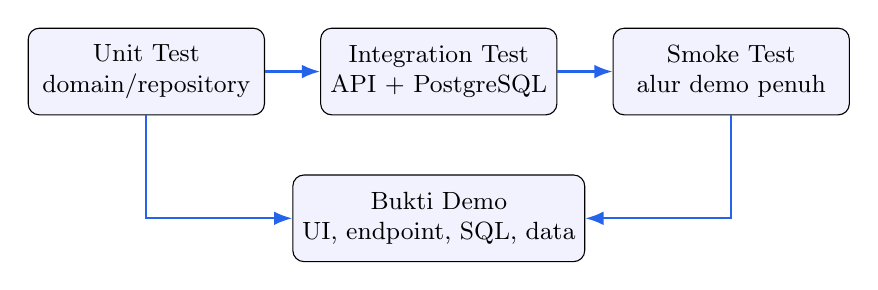
\begin{tikzpicture}[stage/.style={draw, rounded corners, fill=blue!5, align=center, font=\small, minimum width=3.0cm, minimum height=1.1cm}, rel/.style={-Latex, thick, draw=codeblue}]
\node[stage] (unit) {Unit Test\\domain/repository};
\node[stage, right=0.7cm of unit] (integration) {Integration Test\\API + PostgreSQL};
\node[stage, right=0.7cm of integration] (smoke) {Smoke Test\\alur demo penuh};
\node[stage, below=0.75cm of integration] (evidence) {Bukti Demo\\UI, endpoint, SQL, data};
\draw[rel] (unit) -- (integration);
\draw[rel] (integration) -- (smoke);
\draw[rel] (smoke) |- (evidence);
\draw[rel] (unit) |- (evidence);
\end{tikzpicture}
\end{center}
}
\newcommand{\featureflow}[4]{
\begin{center}
\begin{tikzpicture}[flowbox/.style={draw=codeblue, rounded corners=3pt, fill=codebg, align=center, font=\small, text width=2.85cm, minimum height=1.15cm, inner sep=5pt}, flowarrow/.style={-Latex, thick, draw=codeblue}]
\node[flowbox] (ui) {#1};
\node[flowbox, right=0.6cm of ui] (api) {#2};
\node[flowbox, right=0.6cm of api] (db) {#3};
\node[flowbox, right=0.6cm of db] (result) {#4};
\draw[flowarrow] (ui) -- (api);
\draw[flowarrow] (api) -- (db);
\draw[flowarrow] (db) -- (result);
\end{tikzpicture}
\end{center}
}

\newcommand{\docheader}[2]{
\begin{titlepage}
\centering
{\Large\bfseries Prokura HoReCa Supply\par}
\vspace{0.4cm}
{\large Dokumentasi Fitur Microservice Final Project\par}
\vspace{0.8cm}
{\large Workshop Implementasi Rekayasa Perangkat Lunak\par}
\vspace{1.2cm}
{\large\bfseries #1\par}
{\large NIM: #2\par}
\vspace{0.7cm}

\includegraphics[width=4.0cm]{../screenshots/ugm-logo.png}\par
\vspace{0.5cm}
\vfill
{\large Ilmu Komputer\par}
{\large Departemen Ilmu Komputer dan Elektronika (DIKE)\par}
{\large Fakultas Matematika dan Ilmu Pengetahuan Alam\par}
{\large Universitas Gadjah Mada\par}
\vfill
\end{titlepage}
}

\begin{document}
\docheader{Gilbert Nathaniel}{24/533877/PA/22623}

\section*{Peran}
Owner Customer Service. Gilbert bertanggung jawab pada data perusahaan B2B, limit kredit, dan user perusahaan.

\section*{Bukti Microservice}
Customer Service berada di \path{prokura-api/src/services/customer} dan dipasang sebagai service tersendiri melalui \texttt{registerCustomerRoutes}.

\begin{lstlisting}[language=JavaScript]
const serviceRegistry = {
  catalog: registerCatalogRoutes,
  customer: registerCustomerRoutes,
  inventory: registerInventoryRoutes,
  order: registerOrderRoutes,
  reporting: registerReportingRoutes,
};
\end{lstlisting}

Penjelasan: entry \texttt{customer: registerCustomerRoutes} membuktikan Customer Service punya boundary sendiri dan dapat dijalankan sebagai proses service di port \texttt{5103}.

\section*{Tanggung Jawab Fitur}
\begin{enumerate}
\item Manajemen customer/perusahaan.
\item Manajemen user perusahaan.
\end{enumerate}

\section*{Diagram Scenario Flow Fitur}
\subsection*{Manajemen customer/perusahaan}
\featureflow{Admin mengisi\\data perusahaan}{Customer Service\\\texttt{POST /api/companies}}{Insert \texttt{companies}}{Perusahaan muncul\\di daftar klien}

\subsection*{Manajemen user perusahaan}
\featureflow{Admin memilih perusahaan\\dan menambah user}{Customer Service\\\texttt{POST /api/users}}{Insert \texttt{users}\\dengan FK company}{User tampil\\di perusahaan}


\section*{Diagram Tabel yang Ditangani}
\begin{center}
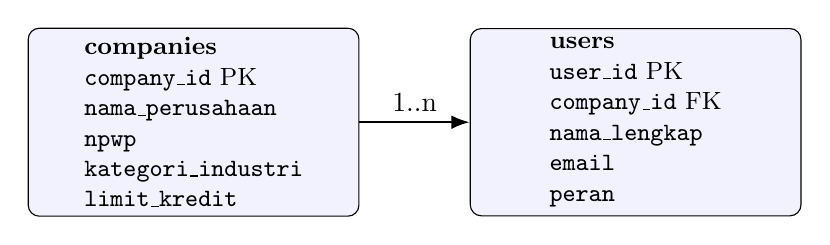
\begin{tikzpicture}[entity/.style={draw, rounded corners, fill=blue!5, align=left, font=\small, minimum width=4.2cm}, rel/.style={-Latex, thick}]
\node[entity] (companies) {\textbf{companies}\\\texttt{company\_id} PK\\\texttt{nama\_perusahaan}\\\texttt{npwp}\\\texttt{kategori\_industri}\\\texttt{limit\_kredit}};
\node[entity, right=1.4cm of companies] (users) {\textbf{users}\\\texttt{user\_id} PK\\\texttt{company\_id} FK\\\texttt{nama\_lengkap}\\\texttt{email}\\\texttt{peran}};
\draw[rel] (companies) -- node[above]{1..n} (users);
\end{tikzpicture}
\end{center}

Penjelasan: Customer Service mengelola master data perusahaan pada tabel \texttt{companies} dan user perusahaan pada tabel \texttt{users}. Satu perusahaan dapat memiliki banyak user.

\section*{Lokasi Kode Program dan Penjelasan}
\subsection*{Route perusahaan}
Lokasi kode: \path{prokura-api/src/services/customer/routes.js}. \texttt{GET /api/companies}: line 11. \texttt{POST /api/companies}: line 20.

\begin{lstlisting}[language=JavaScript]
app.get("/api/companies", async (_req, res) => {
  try {
    const companies = await listCompanies(pool);
    res.json({ success: true, data: companies });
  } catch (error) {
    sendError(res, error, "Gagal mengambil data perusahaan");
  }
});
\end{lstlisting}

Penjelasan: endpoint ini mengembalikan daftar perusahaan untuk UI admin. Data berasal dari repository, bukan dari query langsung di UI.

\begin{lstlisting}[language=JavaScript]
app.post("/api/companies", async (req, res) => {
  try {
    const { nama_perusahaan, npwp, kategori_industri, limit_kredit } = req.body;
    if (!kategori_industri) {
      return res.status(400).json({ success: false, message: "Nama perusahaan dan industri wajib diisi" });
    }

    let companyName;
    try {
      companyName = normalizeCompanyName(nama_perusahaan);
    } catch (error) {
      return res.status(400).json({ success: false, message: error.message });
    }
\end{lstlisting}

Penjelasan: endpoint tambah perusahaan memvalidasi industri dan menormalisasi nama perusahaan. Validasi ini menjaga data master customer tetap rapi.

\subsection*{Route user perusahaan}
Lokasi kode: \path{prokura-api/src/services/customer/routes.js}. \texttt{GET /api/users}: line 46. \texttt{POST /api/users}: line 55.

\begin{lstlisting}[language=JavaScript]
app.get("/api/users", async (req, res) => {
  try {
    const users = await listUsers(pool, req.query.company_id);
    res.json({ success: true, data: users });
  } catch (error) {
    sendError(res, error, "Gagal mengambil pengguna");
  }
});
\end{lstlisting}

Penjelasan: endpoint ini bisa mengambil semua user atau user berdasarkan \texttt{company\_id}. Fitur ini dipakai pada tab manajemen pengguna.

\begin{lstlisting}[language=JavaScript]
app.post("/api/users", async (req, res) => {
  try {
    const { company_id, nama_lengkap, email, peran } = req.body;
    if (!company_id || !nama_lengkap || !email || !peran) {
      return res.status(400).json({ success: false, message: "Data pengguna tidak lengkap" });
    }

    let normalizedEmail;
    try {
      normalizedEmail = validateEmail(email);
    } catch (error) {
      return res.status(400).json({ success: false, message: error.message });
    }
\end{lstlisting}

Penjelasan: endpoint tambah user memastikan company, nama, email, dan peran terisi. Email divalidasi sebelum disimpan.

\subsection*{SQL repository customer}
Lokasi kode: \path{prokura-api/src/services/customer/repository.js}. Insert company: line 13. Insert user: line 52.

\begin{lstlisting}[language=JavaScript]
const { rows } = await pool.query(
  `
    INSERT INTO companies (nama_perusahaan, npwp, kategori_industri, limit_kredit)
    VALUES ($1, $2, $3, $4)
    RETURNING company_id, nama_perusahaan, npwp, kategori_industri, limit_kredit, created_at
  `,
  [
    company.nama_perusahaan,
    company.npwp || null,
    company.kategori_industri,
    company.limit_kredit || 0,
  ],
);
\end{lstlisting}

Penjelasan: query ini menyimpan perusahaan baru dan mengembalikan data lengkap termasuk \texttt{company\_id} dan \texttt{created\_at} untuk ditampilkan di UI.

\begin{lstlisting}[language=JavaScript]
const { rows } = await pool.query(
  `
    INSERT INTO users (company_id, nama_lengkap, email, peran)
    VALUES ($1, $2, $3, $4)
    RETURNING user_id, company_id, nama_lengkap, email, peran
  `,
  [user.company_id, user.nama_lengkap, user.email, user.peran],
);
\end{lstlisting}

Penjelasan: query ini membuat user yang terhubung ke perusahaan melalui \texttt{company\_id}. Return value dipakai sebagai bukti user berhasil dibuat.

\subsection*{UI admin customer}
Lokasi kode: \path{prokura-admin/app3.py}; menu \texttt{Manajemen Klien B2B}: line 683, tabs daftar/tambah/user: line 685, API create company sekitar line 732, API create user sekitar line 769.

Penjelasan: admin menambah perusahaan dan user lewat form Streamlit yang memanggil endpoint Customer Service.

\section*{SQL Query Demo dan Penjelasan}
\subsection*{Query 1: tambah perusahaan}
\begin{lstlisting}[language=SQL]
INSERT INTO companies (nama_perusahaan, npwp, kategori_industri, limit_kredit)
VALUES ('PT Demo Customer', '12.345.678.9-000.111', 'Hotel', 10000000)
RETURNING company_id, nama_perusahaan, npwp, kategori_industri, limit_kredit, created_at;
\end{lstlisting}
Penjelasan: query ini membuat perusahaan B2B baru dengan limit kredit. \texttt{RETURNING} membuktikan perusahaan tersimpan dan menghasilkan \texttt{company\_id}.

\subsection*{Query 2: tambah user perusahaan}
\begin{lstlisting}[language=SQL]
INSERT INTO users (company_id, nama_lengkap, email, peran)
VALUES (1, 'User Demo', 'user.demo@prokura.test', 'Procurement')
RETURNING user_id, company_id, nama_lengkap, email, peran;
\end{lstlisting}
Penjelasan: query ini menambahkan user untuk perusahaan tertentu. \texttt{company\_id} menjadi foreign key yang menghubungkan user dengan customer B2B.

\subsection*{Query 3: lihat user per perusahaan}
\begin{lstlisting}[language=SQL]
SELECT u.user_id, u.company_id, c.nama_perusahaan AS company,
       u.nama_lengkap, u.email, u.peran
FROM users u
JOIN companies c ON u.company_id = c.company_id
WHERE u.company_id = 1
ORDER BY c.nama_perusahaan ASC, u.nama_lengkap ASC;
\end{lstlisting}
Penjelasan: query ini menampilkan user beserta nama perusahaan. Join membantu membuktikan user yang dibuat benar-benar terhubung ke perusahaan yang dipilih.

\section*{Alur Demo}
\subsection*{A. Manajemen customer/perusahaan}
\begin{enumerate}
\item Buka admin \texttt{Manajemen Klien B2B}.
\item Tampilkan daftar perusahaan sebelum penambahan.
\item Masuk tab \texttt{Tambah Klien Baru}.
\item Isi nama perusahaan, NPWP, industri, dan limit kredit.
\item Submit form.
\item Tunjukkan row perusahaan baru di UI dan database.
\end{enumerate}

\subsection*{B. Manajemen user perusahaan}
\begin{enumerate}
\item Masuk tab \texttt{Manajemen Pengguna}.
\item Pilih perusahaan yang baru dibuat.
\item Isi nama user, email, dan peran.
\item Submit form.
\item Tunjukkan user muncul pada tabel perusahaan.
\item Jalankan SQL join user-company untuk membuktikan relasi database.
\end{enumerate}



\section*{Screenshot Demo}
Screenshot berikut menjadi bukti visual bahwa Customer Service sudah terhubung ke panel admin untuk data perusahaan dan user.

\demoscreenshot{../screenshots/gilbert-admin-tambah-perusahaan-1.png}{Demo Gilbert: form tambah perusahaan B2B sebelum data disimpan.}
\demoscreenshot{../screenshots/gilbert-admin-tambah-perusahaan-2.png}{Demo Gilbert: perusahaan B2B berhasil muncul pada daftar klien.}
\demoscreenshot{../screenshots/gilbert-admin-tambah-user.png}{Demo Gilbert: form tambah user perusahaan dan tabel user setelah insert.}

\section*{Bukti Validasi}
Diagram berikut merangkum lapisan validasi yang dipakai sebelum demo: unit test memeriksa logic kecil, integration test membuktikan API dan PostgreSQL berjalan bersama, smoke test menjalankan alur final project end-to-end, lalu bukti demo mengaitkan UI, endpoint, SQL, dan perubahan data.

\validationdiagram

\begin{itemize}
\item Unit test Customer: \path{prokura-api/tests/unit/customer-domain.test.js}.
\item Repository test Customer: \path{prokura-api/tests/unit/repository.test.js}.
\item Integration test membuat company dan user.
\item Smoke test final project membuat company dan user demo.
\end{itemize}

\end{document}
